\chapter{绪论}\label{chap:introduction}
本章介绍本文的研究背景、目的和结果。第一节概括性的介绍多方安全计算问题、协议、程序和验证。第二节举例介绍了多方安全计算程序验证方面的研究情况,并提出本文研究的Wys*程序安全计算函数的编译可行性问题。第三节详细说明了本文研究的具体问题以及基于类型检查的研究方法和对示例程序的测试结果。
\section{背景介绍}
随着互联网技术的普及应用,不同的应用场景都在寻找合适的互联网解决方案。其中一类需要由可信第三方作为中间担保人来保护参与者隐私的诸多实际传统应用和新型网络应用,例如无记名投票、碱基序列比较、数据库的私有查询、隐私集合求交集等,利用多方安全计算技术得以实现在免除第三方中间人的需要的同时满足高隐私保护性,避免由于第三方担保人的失误导致的安全问题和对第三方可信赖程度的担忧。

多方安全计算最早在1982年由姚智期在百万富翁问题中提出。百万富翁问题是两方安全计算问题的一个简单实例,表述为如何在不借助第三个人的情况下,使两个百万富翁比较出谁更富有并且彼此不让对方得知自己的财富数量。姚智期随后提出了解决任意两方安全计算的混淆电路协议(Garbled Circuits Protocol)方法\citep{yao1982protocols}。Goldreich等人将两方计算问题进行拓展,与1987年系统性的阐述了多方安全计算问题,并提出了基于秘密共享(Secret Sharing)的GMW协议\citep{goldreich2019play}(Goldreich-Micali-Wigderson Protocol)。多方安全计算解决的问题是如何使互不信任的参与者,在保证各自隐私数据不被泄漏的情况下,协同计算一个结果依赖于各方隐私数据的函数。SMPC协议发展至今出现了许多高效可靠的技术用于提高SMPC的计算效率,也出现了结合混淆电路和秘密共享两种方案长处的混合协议,专用于开发多方安全计算程序的框架也被开发出来,SMPC得以逐渐在实际问题中应用。

在软件安全领域,对多方安全计算程序的形式化验证也受到了研究者的关注,近年来出现了基于语言的SMPC程序验证方案SecreC\citep{almeida2018enforcing}和Wys*\citep{rastogi2019textsc}。这两种方案从不同的角度对SMPC程序的部分性质进行了验证,虽然各自都有一些缺点,但是为语言层面的SMPC程序验证工作打开了思路。本文以Rastogi等人提出的SMPC程序的领域特定语言Wys*\citep{rastogi2019textsc}为研究对象,Wys*最大的特点是面向程序验证,相比于SecreC\citep{almeida2018enforcing}等其他SMPC验证工作,Wys*依托于F*的逻辑推理和证明能力,能够对程序的计算正确性和安全性进行验证。Wys*是首个SMPC程序的领域特定语言(Domain Specific Language),基于对Wys*的分析发现存在一些有待改进的缺点,其中的一个缺点就是Wys*没有对从代码到电路的编译时可行性进行检查,导致经过验证的Wys*程序在实际运行时可能因为电路编译失败出现运行时错误,这个缺点在SecreC中也同样存在。基于此观察,本文设计开发对Wys*程序中的安全计算函数进行电路编译的可行性进行检查的方法,作为Wys*和SMPC验证的有益补充。
\section{SMPC验证的发展现状}\label{sec:system}
Backes等人\citep{backes2010computationally}早在2010年利用Applied $\pi$-calculus方法对SMPC协议模型进行符号抽象,并基于类型检查的方法提出一种对符号抽象后的SMPC协议模型的正确性进行形式化验证的方法。此方法验证SMPC在协议层面的可靠性,但进行了切实可行的设计实现和实验。 随后Almeida等人\citep{almeida2018enforcing}提出了基于语言的验证SMPC程序隐私数据安全性的验证方法,在Sharemind\citep{bogdanov2008sharemind}安全计算框架中的SecreC(类似C++ 的商业性SMPC语言)基础上,加入特殊的解密操作符declassify,并将数据和运算符都分为public和private类型,然后建立了隐私数据泄漏情况推理系统。SecreC允许设定数据泄漏的阈值函数,在分析SecreC的程序信息流(Information Flow)过程中用于进行检查,验证SecreC编写的SMPC程序对隐私数据的保护程度是否满足所设定的隐私泄漏阈值。Rastogi等人\citep{rastogi2019textsc}提出的Wys*是一种SMPC领域特定语言,Wys*基于F*(由微软研究院和法国国家信息与自动化研究所主导开发的面向验证的函数式语言),继承了F*的逻辑推理功能(Logic Inference),精化类型系统(Refinement Type System)和条件预言(Predicate)等为程序验证服务的功能。Wys*的设计使其能够对SMPC程序的计算正确性、安全性进行证明,同时也兼顾加入了用于开发高性能SMPC程序的特殊功能。

上述提到的主要是基于语言层面进行SMPC验证的工作,这些工作的目的都是验证SMPC程序的安全性质,但是显然不可能包含SMPC程序的所有安全性质,研究的具体内容各有偏向:Backes等人的研究关注SMPC协议模型在协议层面的正确性;Almeida等人的研究关注于SMPC程序在计算时的隐私保护能力,寻求在减少SMPC程序的协议交互,提高SMPC程序性能的同时依然保持合理的数据隐私保护能力;Rastogi等人的研究更关注于Wys*本身的形式化验证,从语言基础的层面保证SMPC程序的计算正确性和安全性。但是各个方案也都有明显的不足之处,以本文研究的Wys*为例,Wys*中使用的电路编译模块和GMW协议模块都不在Rastogi等人的工作的验证范围之内,其他地方也仍有不足,在实际应用中都是不安全的因素。

\section{本文的目的、方法及主要结果}
Rastogi等人的工作开发的Wys*具备进行完整、高效验证SMPC程序的能力,但是本身明显也能看到不足之处。通过对Wys*的设计内容和结构实现的详细分析,我们发现Wys*程序在运行时需要将程序中的安全计算函数编译为布尔电路,但是Wys*没有对这一部分函数进行检查,导致存在程序运行时电路编译失败而出现程序错误的可能,本文因此提出Wys-ckt工具。Wys*程序中的安全计算函数需要被编译为电路,Wys-ckt对这部分函数进行验证,验证这部分函数的语义没有超出Wys*的电路编译能力。Wys-ckt工具保证了经过Wys-ckt验证的程序中的安全计算函数一定能被Wys*顺利的编译为电路,避免了Wys*程序在运行时由于安全计算函数的语义超出的电路编译能力而出现的程序异常。

本文工作在推进时遇到一些难以解决的困难,一方面F*目前仍处于快速迭代中,尚没有公开完整的语法和类型系统,只能从教程和源码中获取主要语法;另一方面,Wys*依赖于特定的F*版本,所依赖的F*版本为非正式版,存在尚未修复的问题。因此,本文将Wys*看作F*的派生语言,根据Rastogi等人发表的与Wys*相关的文献\citep{rastogi2017wys, rastogi2014wysteria,rastogi2019textsc}中公开的特殊语法及类型,设计和实现了Wys*语言的程序文法分析器、静态类型分析以及电路编译可行性验证系统。

简单的Wys*程序经过F*验证系统的验证之后,几乎不需要修改就能在Wys-ckt中进行电路翻译条件满足性的验证。较为复杂的Wys*程序,由于F*语言设计中计算部分与验证部分保持分离的特点,经过F*的验证之后,将计算部分输入Wys-ckt中也能完成验证。

本文以Wys*中的三个SMPC程序示例:mill,median,psi为例进行实验。mill是一个百万富翁问题的程序实例;median是一个两方各输入两个整数求中位数的程序实例;psi是一个集合求交集问题的程序实例。我们在一台主频为2.30GHz的i5-6300HQ处理器平台上运行的Ubuntu 18.04系统当中对这三个程序示例的进行测试。测试结果如表\ref{tab:result}所示, 表中行数一栏代表不同程序源代码的行数,时间一栏代表Wys-ckt对一个程序进行三次分析验证需要花费时间的平均值,最大占用内存代表验证一个程序期间Wys-ckt占用内存的最大值,结果一栏表示Wys-ckt对程序的类型分析结果和验证结果是否符合预期。
\begin{table}[!htbp]
    \caption{Wys-ckt测试结果}
    \label{tab:result}
    \centering
    \footnotesize% fontsize
    \setlength{\tabcolsep}{4pt}% column separation
    \renewcommand{\arraystretch}{1.2}%row space 
    \begin{tabular}{lccccc}
        \hline
        程序示例 & 行数 & 时间(秒) & 最大占用内存(MB) & 结果 \\
        %\cline{2-9}% partial hline from column i to column j
        \hline
        mill   & $21$ & $0.005$ & $2.97$ & 正确 \\
        median & $51$ & $0.007$ & $3.11$ & 正确 \\
        psi    & $46$ & $0.007$ & $2.95$ & 正确 \\
        \hline
    \end{tabular}
\end{table}

根据\ref{tab:result}中的结果,Wys-ckt的实际表现符合设计预期。Wys-ckt的运行时间包含对整个输入程序的分析和对安全计算函数的验证两部分。因此随着输入程序规模的增长,Wys-ckt的运行时间随之增加。Wys-ckt占用的内存主要来自类型分析时存储的数据信息,随着输入程序中表达式数量的增加,Wys-ckt占用的内存呈现近似线性的增长。
\begin{figure}[!htbp]
    \centering
    \begin{subfigure}[b]{0.4\textwidth}
      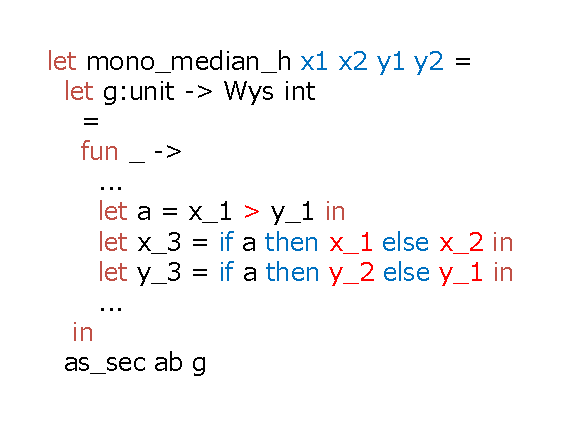
\includegraphics[width=\textwidth]{code.pdf}
      \caption{}
      \label{fig:code}
    \end{subfigure}%
    ~%add desired spacing
    \begin{subfigure}[b]{0.4\textwidth}
      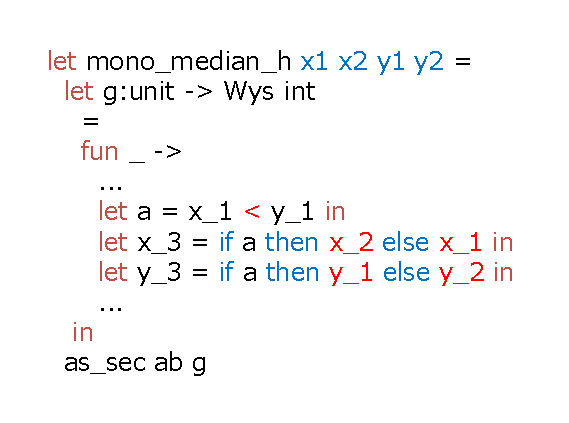
\includegraphics[width=\textwidth]{code2.pdf}
      \caption{}
      \label{fig:code2}
    \end{subfigure}
    \caption{(a) median原始代码的一部分,(b) 经过修改的median代码.}
    \label{fig:codeall}
\end{figure}

表\ref{tab:result}中三个例子都是Wys*提供的能够经过验证编译的程序,Wys-ckt的测试结果也正确的分析出了程序中语法树、类型与验证结果。接下来展示一个有电路编译错误的例子,图\ref{fig:code}中的内容是一段median例子中安全计算函数的一部分代码,将这段代码稍微修改得到图\ref{fig:code2}中的代码,两段代码的6-8行的内容不完全相同,但是却有完全等价的逻辑功能。将median中的图\ref{fig:code}展示的这部分代码修改为图\ref{fig:code2}中的内容后,新的median程序依然能够通过F*的验证,但是在运行时却会因为第6行的布尔比较操作符(<)不在Wys*的电路接受的操作符之内,会产生程序错误。类似这样的错误在一个不熟悉Wys*内部实现细节的多方安全计算程序开发人员的开发过程中是十分容易出现的。但是新的median经过Wys-ckt验证时,Wys-ckt可以发现这个问题并给出警告。通过以上对两种不同类型的例子的实验,证明了Wys-ckt工具的程序实现达到了Wys-ckt设计的预期功能,拥有验证Wys*程序中安全计算函数电路编译可行性的能力,Wys-ckt设计的验证条件保证了一个经过Wys-ckt验证的程序中的安全计算函数一定没有超过Wys*的电路编译能力。
\section{论文的结构}
本文的第二章是预备知识,详细介绍多方安全计算程序的执行过程,领域特定语言Wys*的特性和Wys*进行电路翻译的方法。

第三章重点介绍Wys-ckt的整个设计方案。第三章中将Wys*与F*进行合并,构建了本文研究的Wys*较为形式的语法系统,并且根据类型系统设计的原则将Wys*的特性加入进经典的类型系统当中,最后基于类型设计了电路翻译条件的验证系统,从理论上完成了Wys-ckt的构建。

第四章介绍本文如何将Wys-ckt的理论系统进行实现。Wys-ckt的实现基于O-caml,与F*同属ML家族,利用模式匹配特性可以方便的构建分析作用的代码。本文实现的大部分篇幅用于构建一个完善的拥有类型系统的语法树,然后按照第三章设计的验证模式进行验证。 
